\subsection{Conceptual Model} \label{ConsMod}
\Cref{ConceptualModelPicture} shows a conceptual model between different domains of requirements and actions. This conceptual model is created to give an overview of what has been defined in the rest of \nameref{ModDev} in \cref{ModDev}. The four boxes with sharp corners are seen as domains, some of which have been used in the scenario corpus. Recipes has not been used as one of the main domains in scenario corpus, but includes the information need to cook the specific recipes. Another domain that is not seen in \cref{ConceptualModelPicture} is the general domain, this domain contain requirements which are not directly influencing or needed in in the other domains, which is why it is not included in the model. the other boxes with the soft corners are requirements to the different domains, lastly the arrows with text are actions that sets new requirements.

\begin{figure}[H]
	\centering
    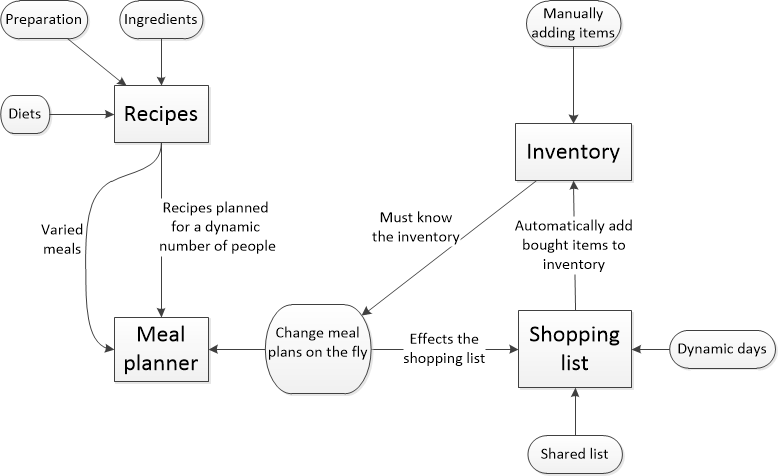
\includegraphics[width=1\textwidth]{Grafik/conceptualModel}
	\caption{Conceptual Model}
	\label{ConceptualModelPicture}
\end{figure}